\documentclass{standalone}

\usepackage{tikz}
\usetikzlibrary{matrix}
\usepackage{times} % To change font to times
\usetikzlibrary{decorations.markings,positioning,shapes,arrows, decorations.pathreplacing}
\usepackage{circuitikz}

\tikzset{font=\Large}
\tikzset{
basic/.style  = {draw, align=center, rectangle},
Gain/.style = {draw, align=center, isosceles triangle, isosceles triangle apex angle=40, scale=0.8},
sum/.style = {draw, circle, scale=1, font={\small +}},
convert/.style 2 args={
	draw,
	minimum size=1cm,
	append after command={
	\pgfextra{
		\pgfinterruptpath
		\path (\tikzlastnode.north west)
		node[inner sep=2pt,anchor=north west]{#1};
		\path (\tikzlastnode.south east)
		node[inner sep=2pt,anchor=south east]{#2};
		\draw (\tikzlastnode.south west) -- (\tikzlastnode.north east);
		\endpgfinterruptpath
	}
	},
}
}

\begin{document}
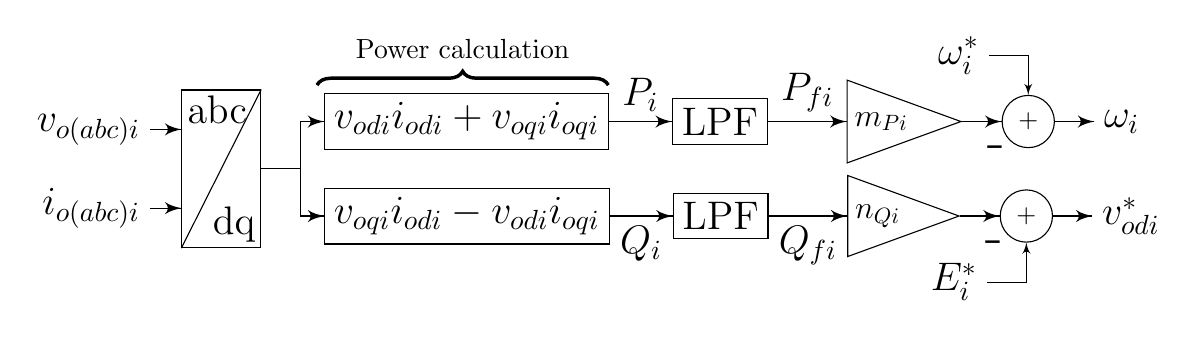
\begin{tikzpicture}[node distance = 1.7cm and 0.8cm, >=latex']

	\node[convert={abc}{dq}, minimum height = 2cm] (abcdq) {};
	\node[basic, right =of abcdq, yshift = 0.6cm] (Pi) {$v_{odi}i_{odi}+v_{oqi}i_{oqi}$};
	\node[basic, right =of abcdq, yshift = -0.6cm] (Qi) {$v_{oqi}i_{odi}-v_{odi}i_{oqi}$};
	\node[basic, right =of Pi] (LPF_P) {LPF};
	\node[basic, right =of Qi] (LPF_Q) {LPF};
	\node[Gain, right =1cm of LPF_P] (mPi) {$m_{Pi}$};
	\node[Gain, right =1cm of LPF_Q] (nQi) {$n_{Qi}$};
	\node[sum, right =0.5cm of mPi] (sumP) {};
	\node[sum, right =0.5cm of nQi] (sumQ) {};

	\draw[decoration={markings,mark=at position 1 with     {\arrow[scale=1.5,>=latex']{>}}},postaction={decorate}] ($(abcdq.west)+(-0.4,0.5)$) -- node[at start, left]{$v_{o(abc)i}$} ++(0.4,0);
	\draw[decoration={markings,mark=at position 1 with     {\arrow[scale=1.5,>=latex']{>}}},postaction={decorate}] ($(abcdq.west)+(-0.4,-0.5)$) -- node[at start, left]{$i_{o(abc)i}$} ++(0.4,0);
	\draw[decoration={markings,mark=at position 1 with     {\arrow[scale=1.5,>=latex']{>}}},postaction={decorate}] (abcdq.east) -- ++(0.5,0) |- (Pi.west);
	\draw[decoration={markings,mark=at position 1 with     {\arrow[scale=1.5,>=latex']{>}}},postaction={decorate}] (abcdq.east)-- ++(0.5,0) |- (Qi.west);
	\draw[decoration={markings,mark=at position 1 with     {\arrow[scale=1.5,>=latex']{>}}},postaction={decorate}] (Pi.east) -- node[midway, above]{$P_i$} (LPF_P.west);
	\draw[decoration={markings,mark=at position 1 with     {\arrow[scale=1.5,>=latex']{>}}},postaction={decorate}] (Qi.east) -- node[midway, below]{$Q_i$} (LPF_Q.west);
	\draw[decoration={markings,mark=at position 1 with     {\arrow[scale=1.5,>=latex']{>}}},postaction={decorate}] (LPF_P.east) -- node[midway, above]{$P_{fi}$} (mPi.west);
	\draw[decoration={markings,mark=at position 1 with     {\arrow[scale=1.5,>=latex']{>}}},postaction={decorate}] (LPF_Q.east) -- node[midway, below]{$Q_{fi}$} (nQi.west);
	\draw[decoration={markings,mark=at position 1 with     {\arrow[scale=1.5,>=latex']{>}}},postaction={decorate}] (mPi.east) -- node[pos=0.85, yshift=-0.05cm, below]{\huge -} (sumP.west);
	\draw[decoration={markings,mark=at position 1 with     {\arrow[scale=1.5,>=latex']{>}}},postaction={decorate}] (nQi.east) -- node[pos=0.85, yshift=-0.05cm, below]{\huge -} (sumQ.west);
	\draw[<-] (sumP.north) |- node[at end, left]{$\omega_i^*$} ++(-0.5,0.5);
	\draw[<-] (sumQ.south) |- node[at end, left]{$E_i^*$} ++(-0.5,-0.5);
	\draw[decoration={markings,mark=at position 1 with     {\arrow[scale=1.5,>=latex']{>}}},postaction={decorate}] (sumP.east) -- node[at end, right]{$\omega_i$} ++(0.5,0);
	\draw[decoration={markings,mark=at position 1 with     {\arrow[scale=1.5,>=latex']{>}}},postaction={decorate}] (sumQ.east) -- node[at end, right]{$v_{odi}^*$} ++(0.5,0);
    \draw[decorate, decoration = { brace, amplitude=5pt}, line width=1.25pt] ($(Pi.north)+(-1.9,0.1)$) -- node[midway, above, yshift=0.2cm]{\normalsize Power calculation} ++(3.7,0);

\end{tikzpicture}


\end{document}